\tab Un branch este o ramura independenta de dezvoltare.Avantajul este ca permite izolarea lucrului de lucrul celalorlalti membrii ai echipei. \\
\textbf{Crearea} unui \textbf{branch} se face cu ajutorul comenzii \textbf{git branch "NameOfTheBranch"}.\\
In mod implicit , branch-ul Git-ului este \textbf{Master}. Astfel, la creearea unui nou branch , si cind le vom afisa, vom avea 2 branc-uri : cel implicit si cel nou creat. In mod implicit, lucreaza Master, dar cind avem nevoie sa lucram pe alta ramura atunci facem switch cu comanda \textbf{git checkout -b "name"}. In continuare am demonstrat crearea,aratarea listei de ramuri , trecerea de la o ramura la alta si stergerea.\\
\begin{figure}[h]
\centering
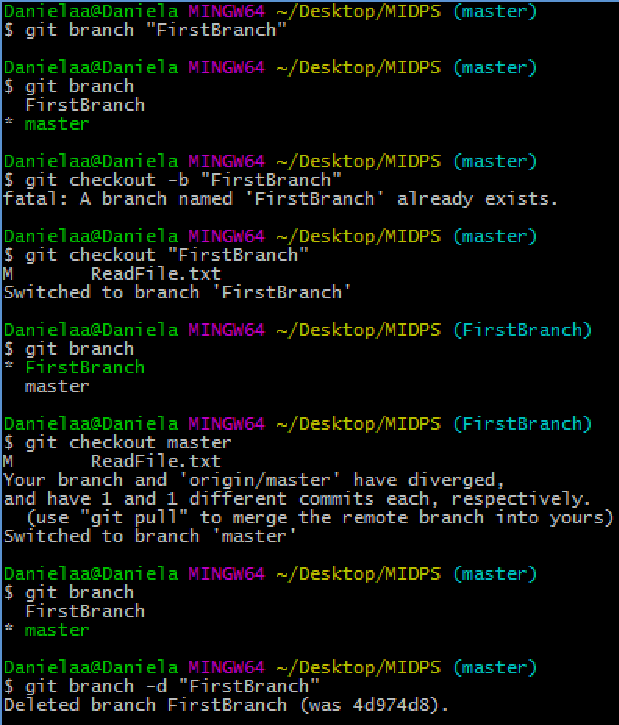
\includegraphics[scale=1]{FirstBranch}
\end{figure}

\clearpage

Facem commit la primul branch creat : 
\begin{figure}[h]
\centering
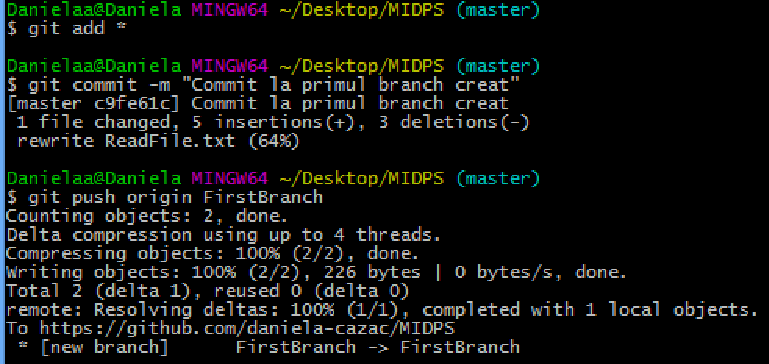
\includegraphics[scale=1]{commitFirstBranch}
\end{figure}

\clearpage